\documentclass[11pt,a4paper]{article}
\usepackage[polish]{babel}
\usepackage[utf8]{inputenc}
\usepackage{polski}
\usepackage[T1]{fontenc}
\usepackage{ae,aecompl}
\frenchspacing
\usepackage[margin=2cm]{geometry}
\usepackage{graphicx}
\usepackage{float}
\usepackage{hyperref}
\usepackage{amsmath}
\usepackage{listings}
\usepackage{color}
\lstset{
        basicstyle=\ttfamily,
        language=C,
        frame=single,
        keywordstyle=\color[rgb]{0,0,1},
        commentstyle=\color[rgb]{0.133,0.545,0.133},
        stringstyle=\color[rgb]{0.627,0.126,0.941},
        columns=flexible,
}

\begin{document}
\title{\LARGE  Projekt nr 2 \\ \vspace{0.4cm} \textbf{Monte Carlo - rozkład temperatury w 2-D}}
\author{Michał Drobniak, 
 Marcin Piłat }
\date{Maj 2013}
\maketitle

\vfill
\begin{figure}[H]
\begin{center}

\includegraphics[width=0.7\textwidth]{agh_nzw_s_pl_1w_wbr_rgb_150ppi.jpg}
\end{center}
\end{figure}
\newpage

\section{Wstęp}
Program służy do obliczania temperatury na płytce dwuwymiarowej w oparciu o znaną temperaturę na brzegach za pomocą metody Monte Carlo. Płytkę dzieli się na siatkę o wymiarach N na N i dla każdej kratki oblicza się temperaturę w sposób iteracyjny:
\begin{enumerate}
\item Losowo wybiera kratkę na podstawie kierunku (góra, dół, prawo, lewo)
\item Sprawdza się temperaturę kratki która została wybrana, jeśli jest znana, to dodaje się ją do sumy temperatur, jeśli nie, to wraca się do poprzedniego punktu i szuka się temperatury dla wybranej kratki.
\item Po dotarciu do znanej temperatury dodaje się ją do sumy temperatur
\end{enumerate}
Temperatura danego punktu to suma temperatur podzielona przez ilość iteracji. Iterowanie się kończy, kiedy temperatura staje się zbieżna (różnica pomiędzy kolejnymi obliczonymi temperaturami jest dostatecznie mała).

\section{Opis implementacji algorytmu}
Powyższy algorytm został zaimplementowany z jedną różnicą: na potrzeby wielowątkowości każdy proces oblicza 500 próbek temperatur (niezależnie od tego, czy się zbiegają, czy nie) i następnie oblicza temperaturę. Następnie każdy proces liczy średnią temperatur obliczonych przez wszystkie procesy (AllReduce) i na tej podstawie decyduje, czy kontynuować obliczenia. Sprawdzanie zbieżności temperatury co 500 próbek powoduje, że narzut komunikacyjny pomiędzy procesami nie jest większy niż czas obliczeń.

Obliczone i początkowe temperatury przechowujemy w tablicy o wymiarach N na N. Wszystkie temperatury oprócz brzegowych są zainicjalizowane wartością -1 (można tak zrobić, ponieważ Kelwiny nie przyjmują ujemnych wartości). Brzegowe temperatury są inicjalizowane zgodnie z treścią zadania: trzy ściany $0^{\circ}$ i czwarta $100^{\circ}$. Dlatego znana temperatura to temperatura większa lub równa $0^{\circ}$.

\begin{figure}[H]
\begin{center}
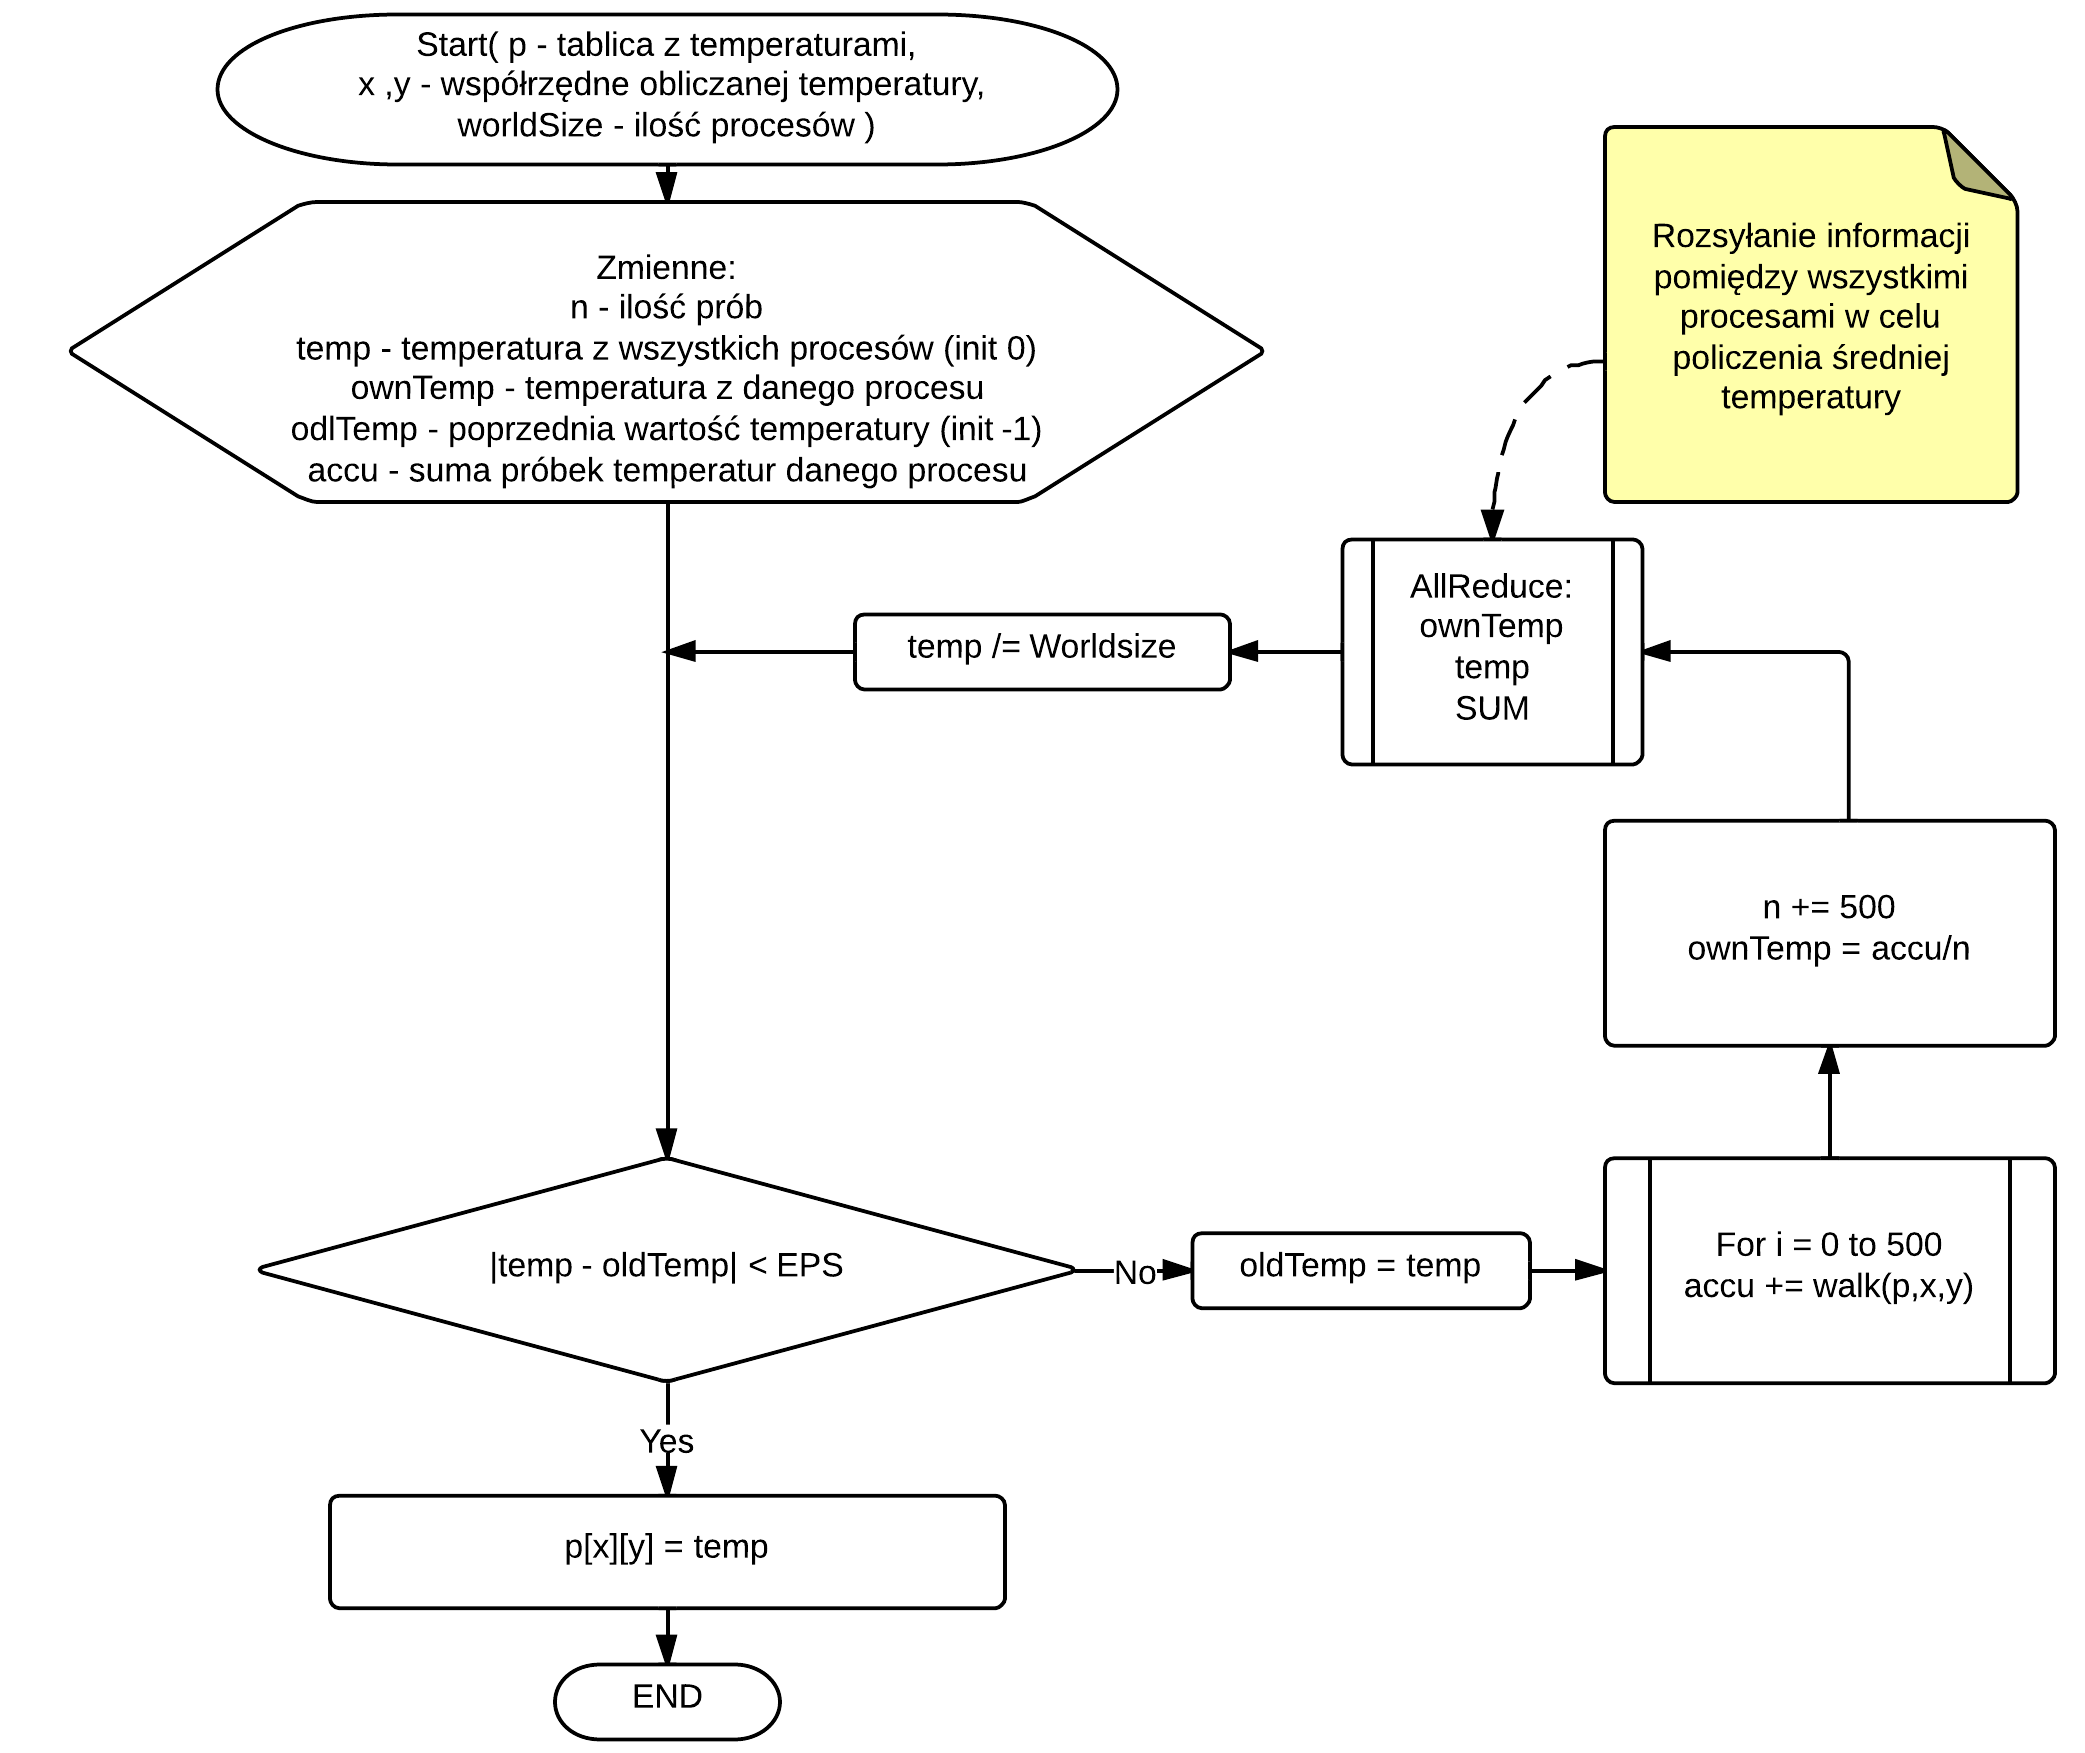
\includegraphics[width=0.7\textwidth]{schemat1.png}
\caption{Schemat blokowy obliczania temperatury w punkcie danym współrzędnymi x i y}
\end{center}
\end{figure}

\begin{figure}[H]
\begin{center}
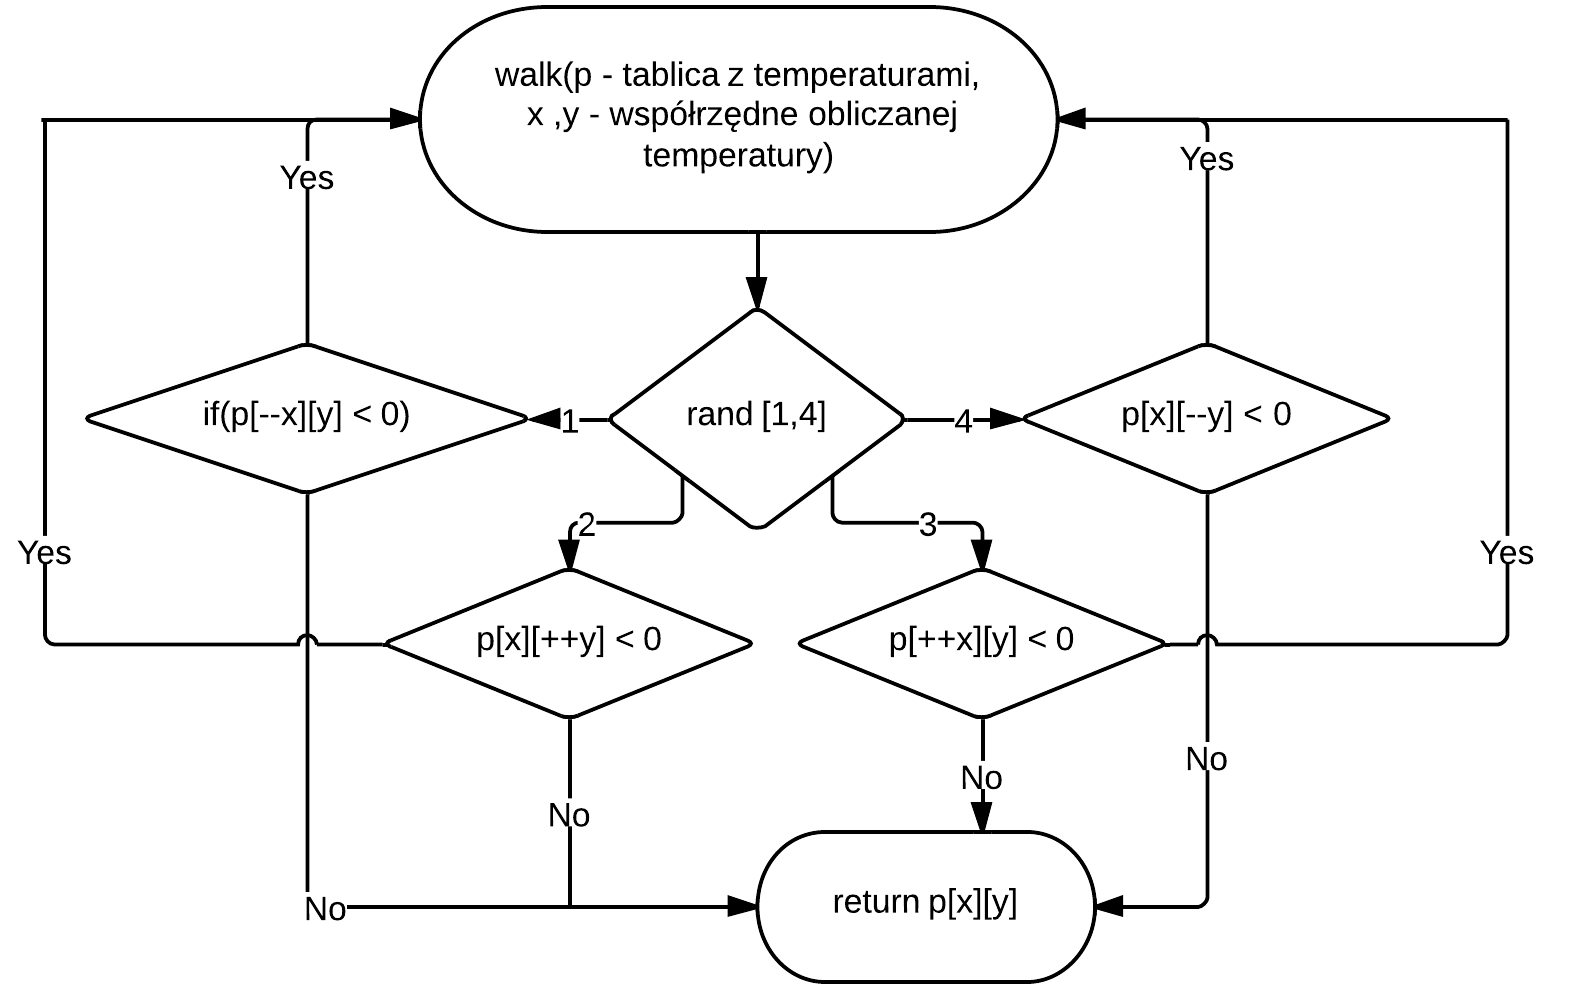
\includegraphics[width=0.7\textwidth]{schemat2.png}
\caption{Schemat blokowy poszukiwania znanej temperatury}
\end{center}
\end{figure}


\end{document}
